\documentclass[11pt,a4paper]{article}

\usepackage{graphicx}
\graphicspath{{Figuras/}}

\usepackage[utf8]{inputenc}
\usepackage[spanish,es-tabla]{babel}
\usepackage[left=2.5cm,right=2.5cm,bottom=2cm,top=2.5cm]{geometry}
\usepackage{titling}
\usepackage{bm}
\usepackage{multirow}
\usepackage{floatrow}
\newfloatcommand{capbtabbox}{table}[][\FBwidth]
\usepackage[table,xcdraw]{xcolor}

\usepackage{blindtext}
\usepackage{verbatim}
\usepackage{amsmath}
\usepackage{amssymb}
\usepackage{textcomp}
\usepackage{bbm}
\usepackage{multicol}
\usepackage{enumitem}
\usepackage{array}
\usepackage{booktabs}
\usepackage{placeins}
\usepackage[hidelinks]{hyperref}

\usepackage[separate-uncertainty = true]{siunitx}
\sisetup{output-decimal-marker = {,}, per-mode=fraction, exponent-product = \cdot}

% Renombre para titulo de referencias / bibliografía
\renewcommand\refname{}

% Bullets para las listas
\renewcommand{\labelitemi}{$\bullet$}
\makeatletter
\def\namedlabel#1#2{\begingroup
    #2%
    \def\@currentlabel{#2}%
    \phantomsection\label{#1}\endgroup}
\makeatother

% Numeración anidada con números
\renewcommand{\labelenumii}{\arabic{enumi}.\arabic{enumii}}
\renewcommand{\labelenumiii}{\arabic{enumi}.\arabic{enumii}.\arabic{enumiii}}
\renewcommand{\labelenumiv}{\arabic{enumi}.\arabic{enumii}.\arabic{enumiii}.\arabic{enumiv}}

\newcommand{\paralelo}{\mathbin{\!/\mkern-5mu/\!}}
\sisetup{exponent-product=\cdot, output-decimal-marker={,}, per-mode=symbol}

\usepackage{fancyhdr}
\usepackage[T1]{fontenc}
\pagestyle{fancy}
\fancyhf{}
\lhead{\textit{Sistema de Aislado Limitado / Total (SAL/T)}}
\rhead{\textit{UBA - Facultad de Ingeniería}}
\cfoot{\thepage}

\setlength{\headheight}{13.6pt}

%%%%%%%%%%%%%%%%%%%%%%%%%%%%%%%%%%%%%%%%%%%

\begin{document}

\pagenumbering{gobble}
\DeclareSIUnit{\div}{div}
\DeclareSIUnit{\Sa}{Sa}

\begin{titlepage}	
	\centering

	%\vspace*{0.3cm}	

     \Large{\textsc{Universidad de Buenos Aires}}\\ 
	\Large{\textsc{Facultad de Ingeniería}}\\ 
	\vspace*{1.4cm}	

	\begin{figure}[h]
		\centering
		
\includegraphics[width=3.5cm]{img/logo_fiuba.pdf} 	
	\end{figure}
	\vspace*{1cm}

\Huge{\textsc{86.00 Tesis de Ingeniería Electrónica - Plan de trabajo \\}}\vspace{.5cm}
	
	\newcommand{\LargoDeBarra}{1}  % Ajustar
	
	\rule{\LargoDeBarra\linewidth}{0.3 mm} \\[0.1 cm]
	\huge{\textbf{Rediseño e implementación de un Sistema de Aislado Limitado / Total (SAL/T) para trenes}} \\[-0.3 cm]
	\rule{\LargoDeBarra\linewidth}{0.3 mm}
	\vspace*{0.5cm}
	
	\begin{table}[htb]
    \begin{tabular}{llcrr} \toprule
        Rol & Integrante              & Padrón    & Correo electrónico  & Teléfono  \\\midrule
        Alumno & Anus, Martín     &    101033  & manus@fi.uba.ar & +54 11 6711-8857 \\\midrule
        Director & Lutenberg, Ariel     &    -  & alutenb@fi.uba.ar  & +54 11 5844-3749 \\\midrule
        Co-director & Gomez, Pablo     &    -  & pgomez@fi.uba.ar & +54 11 6905-2435  \\\midrule
        Co-director & Laiuppa, Adrián     &    -  & alaiuppa@gmail.com & +54 291 643-4357 
        \\\bottomrule
    \end{tabular}
    \end{table}
	\vspace{1cm}
	
	\textsc{\large{Fecha de presentación: 20/04/2024\\}} \medskip
 \textsc{\large{Modalidad de trabajo: Tesis\\}} 

\end{titlepage}

\newpage

\tableofcontents

\newpage

% -------------------------------------------------------------------------------

\setcounter{page}{1}
\pagenumbering{arabic}


\section{Descripción}

Las formaciones ferroviarias cuentan con varios Sistemas Instrumentados de Seguridad (SIS) a bordo con el objetivo de supervisar el correcto funcionamiento de los subsistemas críticos como por ejemplo, la protección de coche a la deriva, el sistema de hombre vivo o la seguridad de puertas. \\

Estos sistemas están diseñados para que, ante la detección de una falla crítica, se produzca la detención de la formación de manera inmediata. Esto se logra controlando las señales de Corte de Tracción (CT) y de Freno de Emergencia (FE). En esta situación, la formación puede ser remolcada o bien, desactivar todos los SIS bajo estricta supervisión y continuar andando con el control manual del conductor hasta una estación cercana para descender a los pasajeros y luego a un taller para ser reparada. \\

El Sistema de Aislamiento Limitado/Total, por sus siglas SAL/T, es un equipo que permite una circulación controlada y más segura de la formación cuando uno de los SIS se encuentra en falla. Al  activar el Modo Aislado Limitado (MAL), el SAL/T va a deshabilitar solamente el SIS que está en fallo y controlar las señales de CT y FE para poder continuar con la circulación de la formación. Para hacerlo de manera segura, el SAL/T va a contar con múltiples fuentes de medición de la velocidad de la formación y va a activar las señales de CT y FE para frenarla en caso de que se excedan los límites estipulados. En el Modo Aislado Total (MAT), se libera la velocidad de precaución y puede ser solamente aplicado por personal superior en el caso que la formación se encuentre sin pasajeros y muy alejada del centro reparador. Ambas activaciones deben ser registradas dentro del equipo así como también cualquier falla detectada, cambio de configuración en las velocidades permitidas o cualquier evento significativo para la seguridad de la formación.\\

Además, el SAL/T cuenta con otras funcionalidad como la comunicación con el conductor a través de una interfaz donde se muestra el estado de los SIS, la velocidad medida en todo momento y un indicador de la zona donde se encuentra la formación. En caso de no contar con una medición de velocidad válida y activar el MAL, el SAL/T entra en Modo Intermitente (MI) y controla la formación activando y desactivando la tracción y el freno acorde a los perfiles de tiempos preconfigurados según las características de la formación para no exceder ciertas velocidades de precaución. Desde el panel formal, el conductor puede seleccionar distintos perfiles intermitentes.  También, el SAL/T tiene la posibilidad de conectarse con una central operativa para informar su estado y recibir remotamente instrucciones. \\

Este equipo es considerado un sistema crítico ya que, en caso de fallar, puede conllevar pérdidas de vidas humanas o daños importantes tanto de propiedades como del entorno. \\

En el 2019, el Ingeniero Iván Di Vito presentó un prototipo de este sistema con pruebas de campo en los talleres de Trenes Argentinos siguiendo las fases y recomendaciones de la norma UNE-EN 50126 \cite{norma_50126};  ``Aplicaciones ferroviarias. Especificación y demostración de la fiabilidad, la disponibilidad, la mantenibilidad y la seguridad (RAMS)''. En el año 2022, los ingenieros Fernando Iglesias y Matías Sambrizzi realizaron el trabajo “Central Operativa para el SAL/T” donde se desarrolló la central operativa para monitorear, controlar y configurar múltiples formaciones equipadas con el SAL/T de manera remota desde un centro de operaciones. Ambos trabajos fueron desarrollados con el acompañamiento del Grupo de Investigación en Calidad y Seguridad de las Aplicaciones Ferroviarias (GICSAFe) como trabajo final de grado de Ingeniería Electrónica en la Universidad de Buenos Aires teniendo como directores al Dr. Ing. Ariel Lutenberg y al Dr. Ing. Pablo Gomez. \\

En este trabajo, se busca hacer un rediseño del prototipo del SAL/T implementando algunas mejoras sugeridas por Trenes Argentinos en el pliego de especificaciones técnicas ET.SO.No 046/18–E3 del 2022, utilizando un microcontrolador y componentes más modernos y un firmware basado en un sistema operativo de tiempo real que resulte más portable que el actual. A continuación se muestra un diagrama en bloques del sistema a desarrollar: 


\begin{figure}[H]
    \centering
    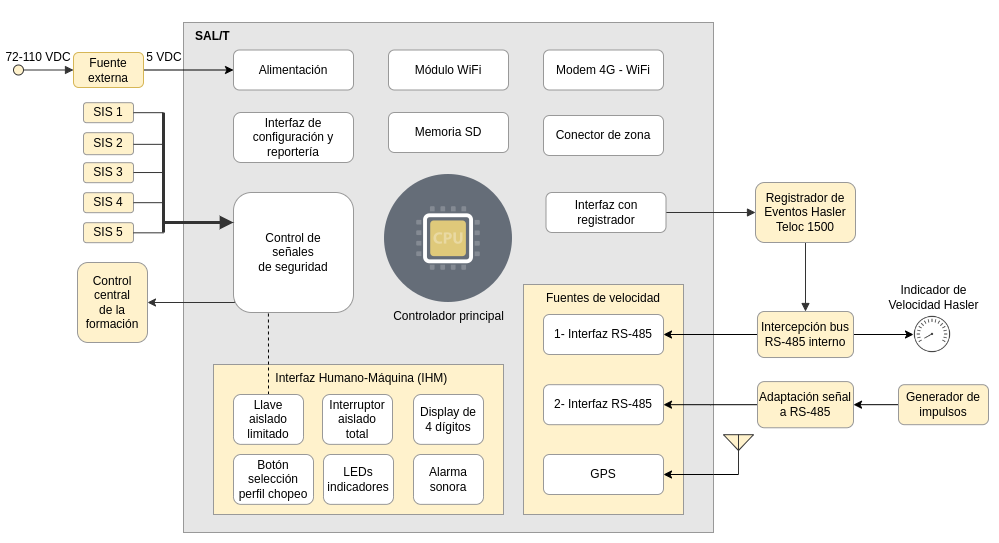
\includegraphics[width=\linewidth]{img/diagrama_bloques.png}
    \caption{Diagrama en bloques del SAL/T}
    \label{fig:block_diagram}
\end{figure}

También se muestra la interfaz humano-máquina (IHM) diseñada para comunicarse con el conductor de la formación:

\begin{figure}[H]
    \centering
    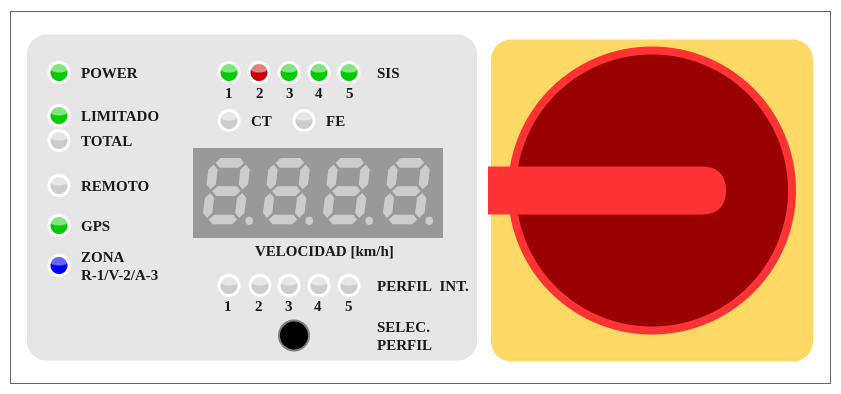
\includegraphics[width=\linewidth]{img/panel_frontal.png}
    \caption{Interfaz humano-máquina del SAL/T}
    \label{fig:him}
\end{figure}
\section{Antecedentes}

El Grupo de Investigación en Calidad y Seguridad de las Aplicaciones Ferroviarias (GICSAFe) fue creado en 2017 en el marco del Consejo Nacional de Investigaciones Científicas y Técnicas (CONICET) de la República Argentina \cite{gicasfe}. En el grupo participan investigadores, docentes y alumnos de diferentes instituciones públicas argentinas quienes realizan desarrollos de sistemas electrónicos e informáticas para aplicaciones ferroviarias relacionadas con la seguridad. Muchos de los prototipos desarrollados son instalados y entregados junto a toda la documentación, respetando normas internacionales de seguridad, para luego transferir el derecho de uso, fabricación y mantenimiento a los clientes. \\

La empresa estatal Trenes Argentinos Operaciones \cite{trenes_arg} encargó al grupo CONICET-GICSAFe el desarrollo de un prototipo del SAL/T en el año 2017. El ingeniero Iván Di Vito, en ese momento estudiante de la carrera de Ingeniería Electrónica en la UBA y allegado al grupo de investigación tomó el proyecto que finalizaría en el año 2019 con la entrega de un prototipo funcional del SAL/T luego de varias pruebas de campo en los talleres de Trenes Argentinos junto a toda la documentación requeridas por las normas de seguridad ferroviarias para este tipo de desarrollos \cite{salt_ivan}. El trabajo realizado incluyó el relevamiento de los requerimientos del proyecto, el desarrollo conceptual de la solución propuesta, el diseño e implementación del hardware y firmware, la puesta en marcha y realización de pruebas de campo de un prototipo funcional. El mismo se realizó de acuerdo a la norma UNE-EN 50126, aplicando técnicas de
patrones de diseño de hardware y software \cite{patrones}. Este trabajo fue publicado por el Congreso Argentino de Sistemas Embebidos (CASE) en el año 2019 en la categoría de artículo \cite{salt_case}. \\

En el año 2021, otros dos estudiantes de la carrera de Ingeniería Electrónica de la UBA, Fernando Iglesias y Matias Sambrizzi, emprendieron un proyecto para el desarrollo de la central operativa del SAL/T en el mismo contexto  de acuerdo entre Trenes y CONICET-GICSAFe. El objetivo de dicho proyecto fue desarrollar el software de una central operativa que permita administrar y configurar
de forma remota dispositivos de supervisión de seguridad de formaciones ferroviarias SAL/T \cite{central_op}. Para esto, se implementó un servicio de monitoreo y control que permite visualizar en tiempo real los datos recibidas y enviar comando de control a los dispositivos activos, la gestión de configuración de dispositivos, la base de datos, los componentes de seguridad necesarios para las comunicaciones e información almacenada y la gestión de usuarios y perfiles. \\

\section{Áreas profesionales de relevancia}

Esta Tesis está enmarcada principalmente dentro del área de Sistemas Digitales y Computación, según lo especificado en la versión 2009, Modificación 2018, del plan de estudios de la Carrera de Ingeniería Electrónica de la Facultad de Ingeniería de la Universidad de Buenos Aires \cite{plan_fiuba}. \\

En particular, están vinculadas a este proyecto las siguientes actividades reservadas al tıitulo de Ingeniero Electrónico:
\begin{itemize}
    \item Diseñar, proyectar y calcular hardware y software de sistemas embebidos y dispositivos lógicos programables
    \item Proyectar, dirigir y controlar la construcción, implementación, mantenimiento y operación de lo mencionado anteriormente.
\end{itemize}


De la misma forma, son particularmente relevantes al proyecto los siguientes alcances del titulo de Ingeniero Electrónico: 

\begin{itemize}
    \item Estudio, planificación, proyectos, estudios de factibilidad técnico-económicos, programación, dirección, construcción, instalación, puesta en marcha, operación, ensayo, mediciones, mantenimiento, reparación, modificación, transformación e inspección de:
    \begin{itemize}
        \item Sistemas, subsistemas, equipos, componentes, partes, piezas (Hardware), de procesamiento electrónico de datos en todas sus aplicaciones incluyendo su programación (Software) asociada.
        \item Sistemas, subsistemas, equipos, componentes, partes, piezas que impliquen electrónica, de navegación o señalización o cualquier otra aplicación al movimiento de vehículos terrestres, aéreos, marítimos o de cualquier otro tipo.

    \end{itemize}
\end{itemize}

\section{Objetivos}

\subsection{Objetivos generales}

Se busca diseñar una solución para aumentar la seguridad en las formaciones ferroviarias ante fallas en los Sistemas Instrumentados de Seguridad mediante un mejor control y monitoreo de velocidad de la formación en tiempo real. La solución debe ser compatible con los mecanismos de seguridad y  sistemas instalados actualmente en las formaciones de Trenes Argentinos. 


\subsection{Objetivos particulares}

\begin{itemize}
    \item Rediseñar el sistema SAL/T a partir de los trabajos existentes y el pliego de especificaciones técnicas propuestos por Trenes Argentinos 
    \item Rediseñar el hardware del SAL/T utilizando componentes vigentes en el mercado
    \item Generar un firmware portable basado en un sistema operativo de tiempo real
    \item Construir un prototipo del proyecto y realizar pruebas de funcionamiento en un entorno similar al real
    \item Favorecer el desarrollo de tecnología nacional 
\end{itemize}

\section{Necesidad y soluciones existentes}

La empresa de Trenes Argentinos mencionó en reiteradas oportunidades la disconformidad con la situación actual de las formaciones ferroviarias frente a algún fallo en los Sistemas Instrumentados de Seguridad (SIS) ya que, al entrar alguno de ellos en fallo, obliga a la formación a ser remolcada o, lo que sucede más frecuentemente en la práctica, a continuar hasta la próxima estación para descender a los pasajeros deshabilitando todos los SIS con los que cuenta la formación. Esto presenta una situación de riesgo ya que la formación pasa a depender fuertemente de la manualidad del conductor sin ningún sistema de seguridad monitoreando y asistiendo la conducción. \\

Al mismo tiempo, la empresa no encuentra alternativas comerciales para satisfacer las necesidades de un Sistema de Aislamiento Limitado / Total ya que necesita integrar distintos SIS y fuentes de medición que no son necesariamente del mismo fabricante o con especificaciones genéricas que permitan su fácil integración.  \\

Por estos motivos, Trenes Argentinos solicitó al grupo CONICET-GICSAFe que diseñara un SAL/T a medida para cumplir con los requerimientos específicos de sus formaciones. En 2019 se entregó una primera versión del prototipo que permitía satisfacer las funciones más importantes del sistema. Sin embargo, antes de requerir una versión productiva y fabricable en cantidades, se determinó que faltaban implementar algunas funcionalidades adicionales para que se pueda instalar un SAL/T en las formaciones. El pliego de especificaciones técnicas para la versión completa del SAL/T se encuentra en disponible en \cite{spec}. \\

Los cambios más relevantes mencionados en el documento que dan lugar a rediseñar el prototipo antes de producirlo en masa son: 
\begin{itemize}
    \item Utilización de un microcontrolador de mayor capacidad y más vigente
    \item Generación de un firmware más portable basado en un sistema operativo de tiempo real
    \item Aislamiento del SIS en falla particular en Modo Aislado Limitado sin interrumpir el funcionamiento del resto de los SIS
    \item Selección de distintos perfiles intermitentes desde el panel frontal del SAL/T
    \item Conector de zona para poder determinas distintas zonas de tránsito para la formación y activar cambios en otros sistemas de la formación
    \item Registro interno de eventos para cambios de estado de SIS, activación de modos, excesos de velocidad y activación de señales de Corte de Tracción y Freno de Emergencia
\end{itemize}

\section{Alcance}



El proyecto consiste en diseñar, desarrollar e implementar un nuevo protitpo del SAL/T teniendo en cuenta que se deben agregar nuevas funcionalidades requeridas, que el hardware debe ser actualizado con componentes vigentes y disponibles actualmente en el mercado internacional y que el firmware desarrollado debe estar basado en un sistema operativo de tiempo real que resulte portable. \\

Para establecer los requerimientos del proyecto, se contempló el prototipo preexistente del SAL/T y el pliego de especificaciones técnicas que generó Trenes Argentinos teniendo en consideración las limitaciones de tiempos y presupuesto que hace sentido para un proyecto de fin de carrera de grado. En el \nameref{anexo}, se adjunta un listado con el detalle de los requerimientos considerados para este proyecto.\\

Una vez finalizado el diseño del sistema, el prototipo debe ser fabricado sobre una placa PCB y se deben montar todos los componentes para su correcto funcionamiento. Se deberán realizar pruebas de laboratorio en las condiciones de funcionamiento para verificar que se cumplas todos los requerimientos establecidos. De ser posible, se intentará coordinar con Trenes Argentinos para realizar algunas pruebas de campo en los talleres de la empresa. 


\section{Entregables}

Se presenta a continuación una lista de los entregables del proyecto:

\begin{itemize}
    \item Documento de diseño de circuitos y selección de componentes
    \item Diseño de esquemático y layout de los PCB
    \item Desarrollo de firmware
    \item Prototipo funcional
    \item Documento de pruebas sobre el prototipo
    \item Informe integral del proyecto

    \end{itemize}
\section{Desglose de Tareas}

Para realizar una mejor estimación de la duración del proyecto, es necesario descomponer el proyecto en tareas generales y estas en subtareas.  A continuación, se muestra un listado de todas las tareas necesarias para completar el proyecto con sus duraciones estimadas. 


\begin{enumerate}
    \item Estudio de Factibilidad   (60hs)
    \begin{enumerate}
        \item Lectura de documentos existentes sobre el SAL/T   (20hs)
        \item Lectura pliego de especificaciones técnicas SAL/T (5hs)
        \item Análisis y acuerdo de nuevas funcionalidad a implementar  (25hs)
        \item Entendimiento de código y puesta en marcha de primer prototipo SAL/T  (10hs)
    \end{enumerate}
    \item Diseño general de la solución (45hs)
    \begin{enumerate}
        \item Redacción de requerimientos del proyecto (7hs)
        \item Diseño de bloques de la solución (15hs)
        \item Análisis de comunicaciones entre módulos integrados (8hs)
        \item Análisis de disponibilidad de tiendas para componentes (10hs)
        \item Análisis de fabricantes de PCB (5hs)
    \end{enumerate}
    \item Desarrollo de hardware (255hs)
    \begin{enumerate}
        \item Investigación y selección de microcontrolador y kit de desarrollo (25hs)
        \item Investigación y selección de módulos GPS (10hs)
        \item Investigación y selección de módulos Wifi (10hs)
        \item Diseño de circuito de medición estado SIS (20hs)
        \item Diseño de circuitos RS485 (10hs)
        \item Diseño de panel frontal (15hs)
        \item Diseño circuitos de relé (15hs)
        \item Selección de componentes (40hs)
        \item Armado de esquemáticos (35hs)
        \item Asignación de pines microcontrolador (15hs)
        \item Selección de tecnología de PCB a utilizar (10hs)
        \item Diseño del PCB (50hs)
    \end{enumerate}
    \item Desarrollo de firmware (215hs)
    \begin{enumerate}
        \item Desarrollo conexión Wifi (15hs)
        \item Desarrollo de comunicación con protocolo MQTT (25hs)
        \item Desarrollo comunicación GPS (15hs)
        \item Desarrollo lecturas de velocidad (20hs)
        \item Desarrollo lectura de estados SIS (15hs)
        \item Desarrollo de lógica de perfiles intermitentes (15hs)
        \item Desarrollo de registro de datos local (25hs)
        \item Desarrollo de descarga de reporte de datos (25hs)
        \item Desarrollo de lógica general del sistema (30hs)
        \item Implementación de módulos en sistema operativo de tiempo real (30hs)
    \end{enumerate}
    \item Fabricación del prototipo (55hs)
    \begin{enumerate}
        \item Compra de componentes (10hs)
        \item Ensamblaje de componentes (15hs)
        \item Verificación de continuidad y señales en la placa (10hs)
        \item Pruebas sobre las comunicaciones (20hs)
    \end{enumerate}
    \item Verificación y validación (80hs)
    \begin{enumerate}
        \item Verificación de casos de uso del prototipo (35hs)
        \item Pruebas de integración (30hs)
        \item Validación de los requerimientos (20hs)
    \end{enumerate}
    \item Revisión de documentación (67hs)
    \begin{enumerate}
        \item Planificación del proyecto (15hs)
        \item Redacción del plan de trabajo (12hs)
        \item Documentación técnica del hardware (20hs)
        \item Documentación del código fuente (20hs)
        
    \end{enumerate}
    \item Presentación del proyecto (110hs)
    \begin{enumerate}
        \item Elaboración de diapositivas para la presentación (20hs)
        \item Confección del informe final (90hs)
    \end{enumerate}
\end{enumerate}

En total, se estiman 887 horas de trabajo necesarias para el desarrollo del proyecto. \\

Además, se presenta a modo de referencia, un cronograma con los plazos aproximados para completar cada una de las tareas generales. 


\begin{table}[h]
\begin{center}
\begin{tabular}{|l|l|l|l|l|l|l|l|l|l|l|l|l|}
\hline
\multicolumn{1}{|c|}{} & \multicolumn{12}{c|}{Meses} \\ \cline{2-13} 
\multicolumn{1}{|c|}
    {\multirow{-2}{*}{Tareas}} 
    & 1 & 2 & 3 & 4 & 5 & 6 & 7 & 8 & 9 & 10 & 11 & 12 \\ \hline
Estudio de Factibilidad             &
\cellcolor[HTML]{656565}{\color[HTML]{333333}}  &
                                                &
                                                &
                                                &
                                                &
                                                &
                                                &
                                                &
                                                &
                                                & 
                                                & \\ \hline
Diseño general de la solución                &
                                                &
\cellcolor[HTML]{656565}{\color[HTML]{333333}}  &                      
\cellcolor[HTML]{656565}{\color[HTML]{333333}}  &
                                                &
                                                &
                                                &
                                                &
                                                &
                                                &
                                                &
                                                & \\ \hline
Desarrollo de hardware      &
                                                &
                                                &    
\cellcolor[HTML]{656565}{\color[HTML]{333333}}  &
\cellcolor[HTML]{656565}{\color[HTML]{333333}}  &
\cellcolor[HTML]{656565}{\color[HTML]{333333}}  &
\cellcolor[HTML]{656565}{\color[HTML]{333333}}  &
                                                &
                                                &
                                                &
                                                &
                                                & \\ \hline
Desarrollo de firmware               &
                                                &
                                                &
                                                &
                                                &
                                                &
\cellcolor[HTML]{656565}{\color[HTML]{333333}}  &
\cellcolor[HTML]{656565}{\color[HTML]{333333}}  &
\cellcolor[HTML]{656565}{\color[HTML]{333333}}  &
                                                &
                                                &
                                                & \\ \hline
Fabricación del prototipo                                 &
                                                &
                                                &    
                                                &
                                                &
                                                &
                                                &
                                                &
                                                &
\cellcolor[HTML]{656565}{\color[HTML]{333333}}  &
                                                &
                                                & \\ \hline
Verificación y validación                &
                                                &
                                                &    
                                                &
                                                &
                                                &
                                                &
                                                &
                                                &   
\cellcolor[HTML]{656565}{\color[HTML]{333333}}  &
\cellcolor[HTML]{656565}{\color[HTML]{333333}}  &
                                                & \\ \hline
Revisión de documentación                &
                                                &                          
                                                &
                                                &
                                                &
                                                &
                                                &
                                                &
                                                &
                                                &            
\cellcolor[HTML]{656565}{\color[HTML]{333333}}  &
\cellcolor[HTML]{656565}{\color[HTML]{333333}}  & \\ \hline                                                
Presentación del proyecto                       &
                                                &
                                                &                          
                                                &
                                                &
                                                &
                                                &
                                                &
                                                &
                                                &
\cellcolor[HTML]{656565}{\color[HTML]{333333}}  &
\cellcolor[HTML]{656565}{\color[HTML]{333333}}  &
\cellcolor[HTML]{656565}{\color[HTML]{333333}}  \\ \hline
\end{tabular}
\end{center}
\end{table}


\section{Referencias}


 \begin{thebibliography}{30}

\bibitem{norma_50126}
\textbf{UNE-EN 50126-1}. Aplicaciones ferroviarias. Especificación y demostración de la fiabilidad, la disponibilidad, la mantenibilidad y la seguridad (RAMS). 2005. \href{https://www.une.org/encuentra-tu-norma/busca-tu-norma/norma?c=N0033106}{https://www.une.org/encuentra-tu-norma/busca-tu-norma/norma?c=N0033106}

 \bibitem{gicasfe}
 \textbf{GICSAFe} Grupo de Investigación en Calidad y Seguridad de las Aplicaciones Ferroviarias. \href{https://sites.google.com/view/conicet-gicsafe}{https://sites.google.com/view/conicet-gicsafe}.


 \bibitem{trenes_arg}
 \textbf{Trenes Argentinos} Trenes Argentinos Operaciones, empresa del estado. \href{https://www.argentina.gob.ar/transporte/trenes-argentinos}{https://www.argentina.gob.ar/transporte/trenes-argentinos}.

 \bibitem{salt_ivan}
 \textbf{Di Vito, Iván Mariano, “Aplicación de la técnica de patrones de diseño a la implementación de un Sistema de Aislamiento Limitado/Total ferroviario,”} 2019 \href{https://bibliotecadigital.fi.uba.ar/items/show/18446}{\textit{https://bibliotecadigital.fi.uba.ar/items/show/18446}}.

 \bibitem{patrones}
 \textbf{Ashraf Armoush. “Design Patterns for Safety-Critical Embedded Systems”} RWTH Aachen University. 2010.

 \bibitem{salt_case}
 \textbf{Ivan Mariano Di Vito, Pablo Gomez, Ariel Lutenberg, Adrian Laiuppa “Sistema de supervisión de la seguridad del material ferroviario utilizando patrones de diseño”.} 2019. \href{https://drive.google.com/file/d/1FDtRL4We4daZ7XrJ81sL2f6HrZbYlOuG/view}{\textit{https://drive.google.com/file/d/1FDtRL4We4daZ7XrJ81sL2f6HrZbYlOuG/view}}. 

 
 \bibitem{central_op}
 \textbf{Iglesias Fernando Julio, Sambrizzi Matias,  “Central Operativa para el Sistema de Aislamiento Limitado/Total Ferroviario (SAL/T)“}. Plan de trabajo, 2022. 

 \bibitem{plan_fiuba}
 \textbf{Plan de estudios de Ingeniería Electrónica - Facultad de Ingeniería, Universidad de Buenos Aires}. Plan 2009, modificación 2018. \href{https://cms.fi.uba.ar/uploads/ELECTRONICA_Modificacion_2018_Plan_2009_Ingenieria_Electronica_RCS_1801_18_f22d3d7a5a.pdf}{\textit{https://cms.fi.uba.ar/uploads/ELECTRONICA\_Modificacion\_2018\_Plan\_2009\_Ingenieria\_ Electronica\_RCS\_1801\_18\_f22d3d7a5a.pdf}}. 


 \bibitem{spec}
 \textbf{SISTEMA DE AISLADO LIMITADO / TOTAL (SAL-T)}. ESPECIFICACIÓN TÉCNICA. Bypass Sistemas Instrumentados de Seguridad a Bordo del Material Rodante ET.SO. No 046 /18 – E3. 2022.


 \end{thebibliography}
\section{Anexo}\label{anexo}

\subsection{Detalle de requerimientos}

\begin{enumerate}
    \item Grupo de requerimientos asociados con la interfaz humano-máquina
    \begin{enumerate}
        \item La interfaz debe contar con una llave rotativa para activar el modo aislado limitado.
        \item La interfaz debe mostrar la velocidad media del equipo en km/h con 4 dígitos.
        \item La interfaz debe indicar el estado de la señal de corte de tracción.
        \item La interfaz debe indicar el estado de la señal de freno de emergencia.
        \item La interfaz debe indicar la presencia de un comando remoto de la central operativa.
        \item La interfaz debe indicar el estado del módulo GPS.
        \item La interfaz debe indicar el estado de la alimentación.
        \item La interfaz debe indicar el modo en el que se encuentra el sistema.
        \item La interfaz debe contener un control local por fuera del panel frontal para activar el modo aislado total.
        \item La interfaz debe indicar con un LED RGB en cuál de las 3 zonas geográficas predefinidas se encuentra el material rodante. 
        \item La interfaz debe indicar el estado de los distintas Sistemas Instrumentados de Seguridad conectados al SAL/T con un LED RGB para cada SIS.
        \item La interfaz debe contar con una botonera o switch que permita cambiar el perfil para modo de tracción intermitente.
        \item La interfaz debe indicar el perfil seleccionado para modo de tracción intermitente.
        \item La interfaz debe contener un buzzer interno para indicaciones sonoras.
    \end{enumerate}
       
    \item Grupo de requerimientos asociados a la comunicación con el registrador de eventos
    \begin{enumerate}
        \item El sistema debe informar al registrador de eventos la activación del modo aislado limitado.
        \item El sistema debe informar al registrador de eventos si la alimentación es correcta.
        \item El sistema debe informar al registrador de eventos la activación del freno de emergencia.
        \item El sistema debe informar al registrador de eventos la activación del corte de tracción.
    \end{enumerate}
       
    \item Grupo de requerimientos asociados al registro de datos
    \begin{enumerate}
        \item El sistema debe mantener un registro de datos local donde se registran los siguientes eventos con marca de tiempo:
        \begin{itemize}
            \item Activación/Desactivación del modo aislado limitado
            \item Activación/Desactivación del modo aislado total (local o remota)
            \item Referencia de velocidad adoptada y sus permutaciones 
            \item Cobertura de señal GPS
            \item Ciclos de permiso, corte y freno en modo de tracción intermitente
            \item SIS en fallo
            \item Velocidad desarrollada
            \item Zona de circulación
        \end{itemize}
        \item El sistema debe permitir descargar los datos registrados mediante una interfaz serie 
        \item El sistema debe poder descargar los datos registrados de manera remota 
    \end{enumerate}
       
    \item Grupo de requerimientos asociados a la comunicación con la central operativa
    \begin{enumerate}
        \item El sistema debe informar periódicamente (con un tiempo configurable) su estado a la central operativa a través de la red de datos WiFi.
        \item Debe existir la posibilidad de usar 2 proveedores distintos de datos de manera simultánea.
        \item Debe existir la posibilidad de conectarse alternadamente a más de una red Wifi
        \item El protocolo de comunicación con la central operativa debe ser MQTT.
        \item El sistema debe ser capaz de recibir un comando remoto que anule el corte de tracción y el freno de emergencia bajo cualquier condición (modo aislado total).
        \item El sistema debe ser capaz de recibir un comando remoto que active el corte de tracción y el freno de emergencia bajo cualquier condición (modo parada total).
        \item El sistema debe ser capaz de recibir un comando remoto que active el corte de tracción y anule el freno de emergencia bajo cualquier condición (modo coche en deriva).
        \item El sistema debe ser capaz de recibir un comando remoto que active el corte de tracción y el freno de emergencia de forma intermitente en ciclos de tiempo configurables (modo intermitente).
        \item El sistema debe ser capaz de recibir un comando remoto que cancele cualquier comando remoto vigente.
        \item El sistema debe ser capaz de recibir comandos remotos que modifiquen sus parámetros internos configurables.
        \item Si no se recibe un nuevo comando remoto luego de un tiempo configurable (por defecto 10 segundos, máximo 1 minuto), debe volver al algoritmo de activación de corte de tracción y freno de emergencia por defecto.
        \item Ante un comando remoto recibido, debe enviar una confirmación de recepción que permita a la central operativa decidir si es necesaria o no una retransmisión.
        \item Debe utilizar algún mecanismo de encriptación para el enlace con la central operativa.
    \end{enumerate}
       
    \item Grupo de requerimientos asociados al modo normal de funcionamiento
    \begin{enumerate}
        \item El modo normal el sistema no debe intervenir en el funcionamiento del material rodante (prioridad alta).
        \item El sistema debe obtener en todo momento la mejor estimación posible de la velocidad de la formación.
        \item Debe ser capaz de recibir la velocidad a partir de una señal digital provista por el registrador de eventos Hasler Teloc 1500
        \item Debe ser capaz de calcular la velocidad a partir de un sistema GPS integrado.
        \item Debe ser capaz de calcular la velocidad a partir de un generador de impulsos
        \item El rango de velocidad soportado por el sistema tiene que estar entre 0 y 120 km/h.
        \item La estimación de velocidad debe tener una precisión del 2 % de fondo de escala.
        \item El sistema debe determinar la posición del material rodante para activar un contacto seco de relé según la zona de operación donde se encuentre.
    \end{enumerate}
       
    \item Grupo de requerimientos asociados al modo aislado limitado
    \begin{enumerate}
        \item En modo aislado limitado el sistema debe evitar la aplicación del corte de tracción.
        \item En modo aislado limitado el sistema debe evitar la aplicación del freno de emergencia.
        \item Ante cualquier error interno, el sistema debe dejar de intervenir en la aplicación del corte de tracción.
        \item Ante cualquier error interno, el sistema debe dejar de intervenir en la aplicación del freno de emergencia.
        \item En modo aislado limitado el sistema debe emitir una señal sonora intermitente a través de un buzzer.
        \item En modo aislado limitado el sistema debe evitar que la velocidad del material rodante supere una serie de límites configurados.
        \begin{enumerate}
            \item Si al pasar de modo normal a modo aislado limitado no se cuenta con una estimación de velocidad, debe activar el corte de tracción y el freno de emergencia por 30 segundos.
            \item Si se supera una velocidad configurable (por defecto 30 km/h), debe activar el corte de tracción y emitir una señal sonora continua a través de un buzzer.
            \item Si se supera una velocidad configurable (por defecto 36 km/h), debe activar el freno de emergencia.
            \item na vez aplicado, el corte de tracción debe dejar de aplicarse si la velocidad vuelve a ser menor a una velocidad configurable (por defecto 25 km/h).
            \item Una vez aplicado, el freno de emergencia sólo debe dejar de aplicarse luego de un tiempo configurable (por defecto 30 segundos) desde que se superó el límite.
            \item Si la lectura de velocidad es inválida, debe activar y desactivar el corte de tracción y freno de emergencia de manera alternada en ciclos de tiempo según perfiles preconfigurados (modo de tracción intermitente).
        \end{enumerate}
        \item El sistema debe interactuar con 5 Sistemas Instrumentados de Seguridad.
        \item El sistema debe ser capaz de identificar qué SIS está fallando y aislar solamente este dejando los demás SIS operativos.
        \item El sistema debe medir la posición del material rodante para modificar las velocidades máximas según la zona de operación donde se encuentre.
    \end{enumerate}
       
    \item Grupo de requerimientos asociados al modo aislado total
    \begin{enumerate}
        \item El sistema solo puede acceder a este modo accionando el control local o mediante comando remoto.
        \item En el modo aislado total el sistema debe liberar la velocidad de circulación.
        \item El sistema debe registrar en el registro de datos la activación de este modo.
    \end{enumerate}
       
    \item Grupo de requerimientos asociados al modo de tracción intermitente
    \begin{enumerate}
        \item El sistema solo deberá acceder a este modo cuando se encuentre en modo aislado limitado y no cuente con ninguna medición de velocidad válida.
        \item El sistema debe permitir la configuración remota de distintos perfiles de operación de manera remota en donde se configuran los valores de Tiempo del permiso de Tracción, Tiempo de ciclo en deriva, Cantidad de ciclos antes de aplicar freno y Tiempo de espera antes de comienzo de nuevo ciclo.
    \end{enumerate}
       
    \item Grupo de requerimientos asociados al hardware y al gabinete
    \begin{enumerate}
        \item El sistema utilizará una fuente externa de 5 V de tensión continua que pueda soportar hasta 25W de potencia.
        \item Los conectores deben estar bien identificados para facilitar la correcta conexión
        \item El sistema debe poseer una placa de circuito impreso con el procesador y periféricos necesarios para el procesamiento de las señales del material rodante y una segunda placa para el los elementos necesarios para la interacción con el conductor
        \item El diseño de la placa de circuito impreso debe contemplar las recomendaciones de la norma IPC 2221 a fines de asegurar la manufacturabilidad del equipo. 
    \end{enumerate}
           
    \item Grupo de requerimientos asociados al desarrollo del firmware
    \begin{enumerate}
        \item El desarrollo del software debe contemplar las recomendaciones de las normas UNE-EN 50126 y UNE-EN 50128.
        \item El sistema debe trabajar con un sistema operativo en tiempo real para mejorar el desempeño y la seguridad del equipo.
    \end{enumerate}
\end{enumerate}

\end{document}